%%Target for future reference:
%http://www.journals.elsevier.com/environmental-modelling-and-software/

%Latex Configuration
%Init document class
\documentclass[11pt]{article}
\usepackage[margin=1.25in]{geometry}        

%Package for Authors on Title Page
\usepackage{authblk}

%Double Spacing Package
\usepackage{setspace}

%Biblatex Init
\usepackage[backend=bibtex, style=authoryear, citestyle=authoryear]{biblatex}
\bibliography{geoSimex}

%Figures Init
\usepackage{graphicx}
\graphicspath{ {images/} }

%Enable footnotes in tables
\usepackage{tablefootnote}

%Enable the \text{} command for use in equations
\usepackage{amsmath}

% For importing results
\usepackage{import}

% For formatting simulation results table:
\usepackage{dcolumn}
\usepackage{lscape}
\newcolumntype{M}[1]{>{\centering\arraybackslash}m{#1}}

\newcommand{\specialcell}[2][c]{%
  \begin{tabular}[#1]{@{}l@{}}#2\end{tabular}} 

%Authors and Affiliations
\author[1]{Daniel Runfola}
\author[1]{Robert Marty}
\author[1]{Seth Goodman}
\author[1]{Michael LeFew}
\author[2]{Ariel BenYishay}
\affil[1]{Institute for the Theory and Practice of International Relations, AidData, William and Mary}
\affil[2]{Department of Economics, William and Mary}
\renewcommand\Authands{ and }

%Title
\title{geoSIMEX: A Generalized Approach To Modeling Spatial Imprecision}

%-------------------------------------
%-------------------------------------
%Analysis
%-------------------------------------
%-------------------------------------


\usepackage{Sweave}
\begin{document}
\Sconcordance{concordance:master.tex:master.Rnw:%
1 21 1 1 5 2 1 1 0 9 1}
\Sconcordance{concordance:master.tex:./title.Rnw:ofs 35:%
1 11 1}
\Sconcordance{concordance:master.tex:master.Rnw:ofs 47:%
40 5 1}
\Sconcordance{concordance:master.tex:./abstract.Rnw:ofs 53:%
1 10 1}
\Sconcordance{concordance:master.tex:master.Rnw:ofs 64:%
47 2 1}
\Sconcordance{concordance:master.tex:./introduction.Rnw:ofs 67:%
1 58 1}
\Sconcordance{concordance:master.tex:master.Rnw:ofs 126:%
51 2 1}
\Sconcordance{concordance:master.tex:./dataMethods.Rnw:ofs 129:%
1 183 1}
\Sconcordance{concordance:master.tex:master.Rnw:ofs 313:%
55 2 1}
\Sconcordance{concordance:master.tex:./results.Rnw:ofs 316:%
1 20 1}
\Sconcordance{concordance:master.tex:master.Rnw:ofs 337:%
59 2 1}
\Sconcordance{concordance:master.tex:./discussion.Rnw:ofs 340:%
1 24 1}
\Sconcordance{concordance:master.tex:master.Rnw:ofs 365:%
63 2 1}
\Sconcordance{concordance:master.tex:./conclusion.Rnw:ofs 368:%
1 14 1}
\Sconcordance{concordance:master.tex:master.Rnw:ofs 383:%
67 2 1}
\Sconcordance{concordance:master.tex:./tables.Rnw:ofs 386:%
1 52 1}
\Sconcordance{concordance:master.tex:master.Rnw:ofs 439:%
71 2 1}
\Sconcordance{concordance:master.tex:./figures.Rnw:ofs 442:%
1 12 1 1 5 7 1}
\Sconcordance{concordance:master.tex:master.Rnw:ofs 463:%
75 2 1}
\Sconcordance{concordance:master.tex:./acknowledgements.Rnw:ofs 466:%
1 1 1}
\Sconcordance{concordance:master.tex:master.Rnw:ofs 468:%
79 5 1}


%-------------------------------------
%-------------------------------------
%Paper Sections 
%-------------------------------------
%-------------------------------------

%Title Page (title.Rnw)
\maketitle 
\begin{flushleft}
\textbf{Corresponding Author}:\\
Dr. Daniel Runfola\\
Institute for the Theory and Practice of International Relations, \emph{AidData}\\
427 Scotland Street, Williamsburg, VA 23185\\
Email: dsmillerrunfol@wm.edu
Telephone: 508.316.9109
Fax: 757.221.4650
\end{flushleft}

\newpage

%Toggle spacing for document
\doublespacing

%Abstract (abstract.Rnw)
\section{Abstract}
There is a large and growing set of literature examining how different classes of models can integrate information on spatial imprecision in order to more accurately reflect available data. Here, we present a flexible approach - geoSIMEX - which can provide parameter and error estimates while adjusting for spatial imprecision.
We illustrate this approach through a case study leveraging a novel, publically available dataset recording the location of Chinese aid in Southeast Asia at varying levels of precision.
Using a difference-in-difference modeling approach, we integrate Chinese aid information with satellite derived data on vegetation (NDVI) to examine if Chinese aid has caused an increase or decrease in vegetation.
Following multiple approaches which do not incorporate spatial imprecision, we find that Chinese aid had a negative impact on vegetation; once spatial imprecision was incorporated into our estimates through the geoSIMEX procedure no evidence of impact is found. \\
\\
\textbf{Keywords}: SIMEX, Spatial Uncertainty, Spatial Data Integration, Simulation, Ecological Fallacy\\

\newpage
\section{Software}
Accompanying this analysis, we provide a new software suite for researchers interested in (a) retrieving and integrating spatially-explicit data sources with varying levels of precision, and (b) modeling relationships using this data in a way which corrects for spatial imprecision in the R environment.  This suite - the \textit{geo} framework - is made available online, along with all documentation and code, at http://geo.aiddata.org.  The case study presented in this paper leverages two components of the geo framework - the geo(query) tool - http://geo.aiddata.org/query - and the geoSIMEX R package - https://github.com/itpir/geoSIMEX. The \textit{geo(query)} tool leverages a high performance cluster computing environment to enable dynamic requests and downloads of spatial data by individuals with limited background in GIS, outputting file formats (i.e., CSV) compatible with a wide range of statistical programs.  The geoSIMEX R package is designed explicitly for a large body of researchers examining the impacts of international aid on environmental outcomes, but the main functions are generally adaptable to other use cases. Code for both tools is provided and made available under an open source license; extensive documentation on the use of this software, as well as the ability to download datasets customized for use with this software, can be found at http://geo.aiddata.org.
\newpage

%Introduction
\section{Introduction}
The lack of exact geographic information on where measurements are obtained presents a barrier to research.
This has become increasingly evident as more scholars integrate geographic data from multiple sources - for example, census, satellite, and GPS sources - to try and establish causal or predictive relationships (c.f., \cite{bare_assessing_2015,buntaine_titling_2015,gallo_mapping_2012,andam_measuring_2008,buchanan_impacts_2016,benyishay_indigenous_2016,runfola_migration_2016,runfola_multi-criteria_2015}).
This paper presents a generalizeable approach to integrating information on the precision of geographic data into both linear and non-linear models - geoSIMEX.
We illustrate the capability of geoSIMEX to provide more accurate parameter estimates than traditional approaches through a simulation framework. 
Using a novel dataset, we then apply both tradional models and a geoSIMEX model to examine the causal impact of Chinese aid on vegetation in Southeast Asia.
We use this case study to illustrate the importance of including information on spatial imprecision into analyses.
Finally, we introduce the \textit{geo(query)} tool - with which all data used in this analysis can be retrieved - as well as an accompanying R package - geoSIMEX - for users seeking to incorporate information on spatial imprecision into analyses.

\subsection{Literature}

Past literature has shown that uncertainty in the locations of where measurements are taken can produce biased estimates in empirical analyses (\cite{perez-heydrich_guidelines_2013,rettie_overcoming_1999}). 
For example, \cite{perez-heydrich_guidelines_2013} show that regression coefficients can be biased when using raster data in conjunction with point data, where the true locations of the point data are only known to exist within some 5-10km radius of the measured location. 
One frequently cited ``best practice" to overcome this challenge is to take average raster values within a buffer encompassing where the point could have fallen, instead of the single raster value associated with the point (\cite{perez-heydrich_guidelines_2013, rettie_overcoming_1999}). 
Another practice to address spatial uncertainty is to aggregate to some higher spatial scale where there is no - or, less - spatial uncertainty (\cite{runfola_using_2014,giner_creating_2014,perez-heydrich_guidelines_2013}). 
Yet another is to only use information for which exact (or, otherwise very precise) geographic information is known (\cite{runfola_migration_2016,dreher_aid_2015,runfola_what_2014}).
\par
There are many limitations, assumptions, and biases that these approaches incur.
Most predominant are the challenges highlighted by the large and well-established body of literature illustrating that analyzing data at different levels of aggregation can produce different regression coefficients and correlation coefficients; given the established nature of this literature we do not provide a full review here, but suggest a number of resources for readers new to employing spatial information (see \cite{clark_effects_1976, goodchild_models_2001, selvin_durkheims_1958, gotway_combining_2002, gehlke_certain_1934, cramer_efficient_1964}). 
As a simple example of this concern, using data from the 1930 US census, \cite{robinson_ecological_2009} found a negative correlation between the proportion of immigrants in a state and average literacy levels, but a positive correlation between being an immigrant and literacy level. 
A number of techniques have been proposed to address such biases, but most rely on additional assumptions (or, covariates) to aid in an effective disaggregation of data to finer scales (i.e., \cite{gotway_combining_2002, zhu_combined_2004,oloughlin_can_2000,wong_modifiable_2004}).
\par
The simulation and extrapolation method (SIMEX) provides a solution to address measurement error in covariates (\cite{wang_bias_1998,kuchenhoff_general_2006,li_functional_2003,cook_simulation-extrapolation_1994}) with a minimal set of assumptions and no additional covariate information, but has not previously been applied to spatial imprecision. 
In traditional application, SIMEX leverages the relationship between increasing measurement error and bias following a two step process. 
First, SIMEX simulates additional measurement error to establish a relation between measurement error and covariate bias:
\begin{equation}
X(\lambda) = X + \sqrt{\lambda}U
\end{equation}
where X is the measured covariate, U is the variance of the measurement error and $\lambda$ is a parameter that simulates additional measurement error. 
$\lambda=0$ corresponds to the original amount of measurement error in the measured covariate, X. 
SIMEX uses increasing values of $\lambda$ (e.g., 0.5, 1, 1.5, and 2) to estimate models with simulated amounts of additional measurement error. 
Next, SIMEX estimates a trend between $\lambda$ and the coefficient on X, and uses the trend to extrapolate back to $\lambda = -1$ (point of no measurement error).  In the next section, we describe a novel deriviation of this approach - geoSIMEX - which adapts SIMEX to the case of geographic imprecision.  








%Data and Methods
\section{Methods and Data}
\subsection{Methods}
Two different approaches are followed to illustrate the validity and applicability of the geoSIMEX process.
First, we use a monte carlo simulation procedure to examine the relative accuracy of geoSIMEX as contrasted to other procedures.  
Second, we apply geoSIMEX to a case study of the impact of Chinese aid on environmental outcomes in Southeast Asia to provide an illustrative example of when the geoSIMEX approach might lead a researcher to a different conclusion than traditional approaches.

\subsubsection{geoSIMEX}
In this section, we detail the geoSIMEX approach using an illustrative example, in which we solve the following simplified equation, with hypothetical districts as units of analysis:
\begin{equation}
NDVI = \theta * \text{Chinese aid} + \epsilon
\label{eqn:ndvi_aid}
\end{equation}
in which Chinese aid is measured with spatial imprecision (due to, for example, limited documentation on which district aid is being sent to). 
Through using geoSIMEX we account for this spatial imprecision to accurately estimate the model coefficient $\theta$, as well as relevant metrics of significance. 
\par
In figure \ref{fig:nepalex}, we present a hypothetical country with sixteen districts for which we seek to solve equation \ref{eqn:ndvi_aid}. 
Four of these sixteen units of analysis, districts 5, 6, 7, and 8 are distinguished on the map. 
Within this study area, a hypothetical data set contains three Chinese aid project locations of various levels of spatial precision, projects A, B, and C. 
Project A is assigned a coordinate pair in District 5 and had strong documentation, resulting
in precise geographic information (i.e. an exact latitude and longitude). 
Due to weaker project documentation, location B has a precision level indicating that it could have been allocated anywhere in the region that includes districts 5, 6, 7, and 8, but the exact location is unknown. 
Project C has very uncertain spatial information, such that it may be anywhere in the country. 
\par
The area (in square kilometers) in which each project location may have been allocated is summarized in table \ref{precision_example}.
Using the spatial overlap between each unit of analysis (the sixteen districts) and the known area an aid project might exist in, we calculate a probability that each district contains a given project\footnote{Here, probabilities are only based on geographic overlap, as opposed to integrating other factors which might mediate where aid is allocated. This equation can be modified to incorporate more information on spatial location, thus allowing a researcher to trade off additional assumptions or information about factors that mediate spatial allocation in exchange for higher degrees of spatial precision (i.e., through dasymetric mapping approaches).}:

\begin{equation}\label{eq:overlaps}
V_{t} = \sum_{S}^{s=1}U_{s}\left ( \frac{a_{st}}{\sum_{T}^{t=1}a_{st}} \right )
\end{equation}
\noindent 
These probabilities are used in the below steps of the geoSIMEX procedure to estimate model parameters while accounting for spatial imprecision.
\par
Before geoSIMEX is run, users must calculate the initial level of spatial imprecision in a given dataset, defined by $\lambda$.
To reflect imprecision across a given set of aid projects and a set of units of analysis (i.e., districts), we calculate (\begin{math}\lambda\end{math}) following:

\begin{equation}\label{lambda}
\lambda = \frac{\sum_{i}^{P}Area \ of \ Coverage_i}{\sum_{i}^{P}Total \ Possible \ Area \ of \ Coverage_i}
\end{equation}

\noindent where $i$ is an individual project out of $P$ total Chinese aid projects. 
$Area \ of \ Coverage_i$ is project $i$'s known area of coverage defined by the available documentation - i.e., the geographic area across which a project could be located. 
$Total \ Possible \ Area \ of \ Coverage_i$ is the area of coverage of project $i$ under complete spatial imprecision - e.g., the geographic area of the study area.
\par
If the latitude and longitude of every aid project was known, $\lambda$ would resolve to 0---indicating zero spatial imprecision. 
If spatial data was only available for the entire study area (e.g., aid provided to a country without any indication of where the project was allocated), $\lambda$ would resolve to 1---indicating 100\% spatial uncertainty. 
In practice, combinations of different levels of precision in the documentation of individual aid projects result in $\lambda$ values between these two extremes, resulting in $\lambda$ between 0 and 1, in which larger values indicate higher spatial imprecision across all measurements.
\par
After $\lambda$ is known, the first step of geoSIMEX involves estimating a naive model (which can be of variable functional forms; for illustration we use ordinary least squares regression) using the source data.
In this example case, for each unit of observation (i.e., district), the total dollars of Chinese Aid in equation 2 is estimated by equally spreading aid according to geographic overlap - i.e., dollars from each project are weighted by the size of each district a given dollar could fall in to, and the final value is the weighted sum across all projects for each district.
In figure \ref{fig:steps}, we provide an example of the geoSIMEX procedure applied to a dataset with an initial $\lambda$ value of 0.4; figure \ref{fig:steps}A illustrates the result from this step for the example dataset.
In this figure, the x-axis represents the $\lambda$ value (spatial imprecision) for a dataset, with higher values indicating more imprecision.
The y-axis represents the estimated value of $\theta$ in equation \ref{eqn:ndvi_aid}.
In \ref{fig:steps}a, the orange line represents the 95\% confidence interval of the coefficient on aid in the naive model fit in step 2, this estimate is plotted at $\lambda = 0.4$, following the estimate of spatial imprecision calculated using equation \ref{lambda}. 
The horizontal black line represents the true model coefficient generated for this example ($\theta$ = 1), which the naive model fails to capture.
\par 
In the second step, additional imprecision is simulated by randomly decreasing the spatial precision of information (in this case, the spatial precision with which Chinese aid projects are known), and re-calculating the total dollars of aid for each unit of observation according to the updated areas-of-overlap between each unit and aid project. 
For example, a project that has a measurement with an exact latitude and longitude will randomly be assigned a lower level of spatial precision - i.e., a county, state, or even the entire country. 
Using these new, reduced levels of precision a model is fit in an identical fashion to step 1, and the estimated $\theta$ parameter, standard errors of the model, and $\lambda$ value for a given permutation are saved.
In figure \ref{fig:steps}b, the black points represent individual iterations, with the saved model coefficients ($\theta$, y axis) and their associated $\lambda$ (x axis) values. 
\par
The third step subdivides this set of iterations into four equally-sized bins based on the level of spatial uncertainty ($\lambda$) of the aid variable (e.g., if $\lambda$ values range from 0.4 to 1, coefficients are separated into bins of 0.40-0.55, 0.55-0.70, 0.70-0.85 and 0.85-1.00). 
Average coefficient and $\lambda$ values are calculated within each bin, represented as red dots in figure \ref{fig:steps}c. 
The fourth step (\ref{fig:steps}d) fits a quadratic trend to the average coefficient and lambda values estimated in step 3.  
The trend is then extrapolated back to $\lambda=0$, providing an estimate of $\theta$ with perfect spatial precision. 
In figure \ref{fig:steps}d, the red line represents the extrapolated trend, and the blue dot represents the extrapolated estimate of the coefficient on aid. 
\par 

In the fifth step, the variance and standard errors of these estimates are calculated using a bootstrap procedure. 
An iterative procedure is followed in which a single point from each bin (defined in step 3) is sampled, a quadratic trend is fit on the resulting values, and the trend is extrapolated back to $\lambda$ = 0. 
This process is repeated iteratively to capture as many permutations as is computationally feasible (with the number of iterations defined as $R$). 
In figure \ref{fig:steps}e, each blue line represents one extrapolated trend and $\lambda$ = 0 estimate. 
Following the approach outlined in \cite{burnham_information_2002}, we use this information to explicitly quantify both the original standard errors and the additional error from spatial imprecision:

\begin{equation}\label{variance}
var(\hat{\bar{\theta}}) = \sum_i^R \frac{1}{R} \{ var(\hat{\theta_i}) + (\hat{\theta_i}-\hat{\bar{\theta_i}})^2 \}
\end{equation}

\noindent where $R$ is the number of extrapolated coefficients (in this example, 1000). 
$var(\hat{\theta_i})$ is the standard error of each extrapolated coefficient, calculated by fitting a quadratic trend on the standard error estimates from each bin, extrapolating back to $\lambda=0$, and collecting the resulting standard error value. 
$(\hat{\theta_i}-\hat{\bar{\theta_i}})^2$ captures the remaining variance attributable to spatial uncertainty, based on the range of possible $\theta$ outcmes found in the extrapolation procedure (step 4).  

\subsubsection{Simulations}

We employ a monte carlo simulation procedure to examine the accuracy of geoSIMEX compared to other approaches to handle spatial imprecision. 
Each simulation follows 7 steps:

\begin{enumerate}
\item One of three hypothetical countries with different administrative heirarchices is generated: (1) a country with 60 subcounties, 30 counties, 10 districts, and 2 regions, (2) a country with 120 subcounties, 40 counties, 20 districts, and 5 regions, or (3) a country with 120 subcounties, 60 counties, 30 districts, and 10 regions. Each subcounty is randomly assigned (a) a spatial area, and (b) a probability of recieving aid. 
\item 50 to 250 aid projects are randomly allocated to subcounties, according to the assigned probability of a subcounty receiving aid. 
\item A simulated measurement of NDVI is generating according to equation \ref{eqn:ndvi_aid} (defined as the number of aid projects plus random error).
\item Each aid project is given a code indicating the spatial precision that a researcher might see. Codes range from indicating the project fell within a sub-county (no spatial imprecision), to falling somewhere within a county, district, region, or the country. 
\item For each iteration, based on the spatial precision our hypothetical researcher would have access to the expected value of aid is calculated for each subcounty. For projects with spatial imprecission, aid is disbursed to subcounties based on spatial area, with larger subcounties having a larger probability of receiving aid.\footnote{For example, consider a project where \$1 million was disbursed to either subcounty A (spatial area of 400km) or subcounty B (spatial area 100km). Because subcounty A is four times as large as subcounty B, subcounty A will be assigned four times as much aid from the project as subcounty B. Specifically, subcounty A will be assigned \$800,000 and subcounty B will be assigned \$200,000. Disbursing aid using spatial area assumes that each location (e.g., each sq. kilometer) within a country has an equal chance of receiving aid; this assumption could be modified according to dasymetric mapping approaches if desired by the researcher.}
\item Equation \ref{eqn:ndvi_aid} is estimated using  models that do not incorporate spatial imprecision: the first uses the expected value of aid, and the second only includes aid projects with complete spatial preceision (dropping out other information).
\item Equation \ref{eqn:ndvi_aid} is estimated using models that seek to incorporate spatial imprecision: geoSIMEX and a model averaging approach. In the model averaging approach, subcounties are assigned a probability of receiving aid according to their spatial size, and the expected value of aid is calculated iteratively according to that probability.  500 models are estimated, where the average coefficient is used with the standard error estimated using equation \ref{variance}. This approach is contrasted to the geoSIMEX approach.
\end{enumerate}

This process is repeated approximately 6000 times, and the rate at which each modeling approach is able to capture the true relationship between aid and NDVI is contrasted along two dimensions.  First, we examine the percent of times that each approach captured the true relationship between Chinese aid and NDVI ($\theta$) within a 95\% confidence interval.  Second, we assess the percent of iterations a hypothetical researcher would have identified these results as being statistically significant at the 95\% level.

\subsubsection{Chinese Aid in Southeast Asia}
In an illustrative case study of geoSIMEX, we examine the causal impact that Chinese aid distributed from 2005 to 2010 had on vegetation (measured using NDVI) in Southeast Asia.  
This study leverages a novel dataset on the location of Chinese international aid in Southeast Asia available at varying levels of precision (i.e., the exact location of each aid project is not always known).  
It integrates this information with a variety of other ancillary datasets, including the NASA Long Term Data Record (LTDR); all data sources are summarized in section 4.2.  
Employing geoSIMEX, we use this case study to illustrate the importance of incorporating information on spatial imprecision into analyses.
\par
A difference-in-difference modeling strategy is followed, in which the average of NDVI before aid was allocated (pre-2004) is contrasted to the average of NDVI after aid was allocated (post-2011) for each of 351 districts (see section 4.2 for more information):
\begin{equation}\label{eq:caseStudy}
Y_{i} = \beta_0 + \theta * Aid_{i} + \sum_{k=1}^{n}(\beta_{k} * X_{i})
\end{equation}
Where $Y_{i}$ is the difference in the average forest loss post-2011 and pre-2004 in district $i$; $Aid_{i}$ is the number of aid projects in each district; $X_{i}$ is a vector of control variables; $\beta_{k}$ is a vector of parameters for each beta covariate, and $\theta$ is the estimated impact of aid.
We calculate the initial $\lambda$ value for our dataset following equation \ref{lambda}, and simulate additional spatial imprecision by allocating aid to increasingly coarse units of administration.  
We repeat this analysis using three alternative modeling approaches to contrast their outcomes to geoSIMEX: (1) an ordinary least squares model in which imprecision is ignored (representative of a traditional case of the ecological fallacy), (2) a linear model in which all coarse-resolution data is removed from the dataset, and (3) a Monte Carlo model averaging approach in which hundreds of equally-probable worlds are generated based on the initial dataset, and the average beta coefficient and standard errors are reported.\footnote{It should be noted there are many approaches to model averaging, including AIC weighting, that are not tested in this paper. It is possible some of these alternative approaches may outperform the Monte Carlo procedure presented here.}



\subsection{Data}

In this analysis, we examine the impact of Chinese aid in Southeast Asia, explicitly focusing on second-level administrative units within Cambodia, Laos, Myanmar, Thailand and Vietman.
To conduct this analysis, we leverage a dataset on the location of Chinese aid derived through a methodology designed to Track Underreported Financial Flows (TUFF; \cite{strange_tracking_2015}).
Covariate data is collected from a variety of sources, summarized in table \ref{data_source_table}.
Our outcome measure - fluctuation in NDVI - is derived from the NASA Long Term Data Record (LTDR) dataset.
While relatively coarse resolution, this dataset represents the longest consistent record of NDVI available at the global scale.
To facilitate our difference-in-difference modeling efforts, we further select a number of covariates we believe could also impact shifts in NDVI (other than Chinese aid).
These include:
\begin{enumerate}
\item{Long-term climate data from the University of Delaware, providing precipitation and temperature data at a monthly time-step for the full data record, which is permuted to produce yearly mean, minimum, and maximum values for each project location. (\cite{willmott_terrestrial_2001})}
\item{Population Data is retrieved from CIESIN at Columbia University, specifically leveraging the Gridded Population of the World (GPW) data record.}
\item{Slope and Elevation data are derived from the Shuttle Radar Topography Mission (SRTM). (\cite{farr_shuttle_2007})}
\item{Distance to rivers is calculated based on the USGS Hydrosheds database.}
\item{Distance to roads is calculated based on the Global Roads Open Access Dataset (gRoads), which represents roads circa 2010, though the actual date of datasets is highly variable by country.}
\item{Urban travel time, calculated by the European Commission Joint Research Centre.}
\item{Nighttime Lights are retrieved from the NOAA Earth Observation Group, calculated from the Department of Defense Defense Meteorological Satellite Program (DMSP).  Lights values are temporally intercalibrated following the procedure outlined in \cite{weng_global_2014}.}
\end{enumerate}
Each of these datasets are processed and aggregated according to their average values within each district included in this analysis.  
Further, the size of districts are controlled for to mitigate the challenge of variably-sized districts across the study area.
In cases where covariates were measured at a resolution coarser than the unit of observation, the relative area of overlap was used to generate a weighted mean.









%Results
\section{Results}
\subsection{Simulations}

Table \ref{naive_Vs_geosimex} shows results from the simulation analysis. 
Results are subset according to the spatial imprecesion of the simulated aid data, with each row of results representing simulations grouped according to the simulated uncertainty (the final row summarizes across all results). 
The naive OLS model using the expected value of aid (i.e., ignoring spatial imprecision) captures the true coefficient about 50\% of the time within a 95\% confidence interval when there is low spatial uncertainty ($\lambda < 0.3$), and the ability of OLS to capture the true coefficient declines as spatial imprecesion increases. 
The naive model that omits aid projects measured with spatial uncertainty captures the true coefficient 60\% to 70\% of the time at a 95\% confidence interval, depending on the level of spatial imprecesion in the data. 
The model averaging approach performs well under low levels of spatial imprecession; however, as spatial imprecesion increases the ability for the model averaging approach to capture the true coefficient decreases. 
Under low levels of spatial imprecesion the model averaging approach captures the true coefficient 85\% of the time, but under high levels of spatial imprecession the model captures the true coefficient 46\% of the time. 
\par
The geoSIMEX model outperforms the model averaging approach in its ability to capture the true coefficient at all levels of spatial imprecesion.
At low levels of spatial imprecesion the geoSIMEX model captures the true coefficient 90\% of the time. 
Higher spatial imprecesion leads to larger standard errors in the geoSIMEX model, reflected by the percentage of time the geoSIMEX model captures the true relation as spatial imprecesion grows. 
At high levels of spatial imprecesion ($\lambda > 0.7$), the geoSIMEX model captures the true relation 100\% of the time; however, large standard errors result in geoSIMEX capturing the true relation and statistical significance 0\% of the time.

\subsection{Chinese Aid in Southeast Asia}
We examine the model results from our analysis of the impact of Chinese Aid in Southeast Asia to provide an illustrative example of how accounting for spatial imprecision can lead to substantively different conclusions than alternative modeling approaches.
Table \ref{seresults} summarizes these findings.
In (1) a linear model that ignores spatial imprecision (i.e., commits an ecological fallacy), (2) a linear model that omits imprecise spatial information, and (3) a Monte Carlo model averaging approach, findings suggest that Chinese Aid has contributed to deforestation. Specifically, an additional aid project within a district is associated with a 1.1 to 1.7 percentage point decrease in NDVI (p < 0.05).
However, when the spatial imprecision of the data is explicitly modeled (4), we find that insufficient evidence exists to determine if Chinese Aid has had a positive or negative impact on vegetation (p > 0.1).
\par
Further, leveraging geoSIMEX we seperately estimate the contribution of (1) spatial imprecision and (2) unexplained model variance to the standard errors estimated for $\theta$.
Here, we find that spatial imprecision contributes 98.5\% of the variance around $\theta$, while unexplained model variance contributes 1.5\%.


%Discussion
\section{Discussion}
These results highlight the importance of incorporating spatial imprecision into analytic approaches which seek to establish causal relationships using spatial data.
Under current ``best practice" approaches, a researcher would find that Chinese aid has had a statistically significant, detrimental and causal impact on deforestation in Southeast Asia, even after controlling for a wide variety of potential confounding variables.
This result - which could have strong policy ramifications - is illustrated to have insufficient evidence to support it when the geoSIMEX procedure is followed, largely due to the relatively imprecise nature of the measurements of aid.
Failing to account for spatial imprecision can thus bias results in key ways, and lead researchers to conclusions that may be inaccurate.
Further, we find nearly all (98.5\%) of the unexplained variance can be ascribed to spatial imprecision; this offers compelling evidence that the true relationship between Chinese aid and deforestation could be better understood if more precise spatial information was collected.
\subsection{geoSimex}
Broadly, this paper is related to papers that seek to overcome issues related to the Ecological Fallacy - i.e., the fallacy of measuring data at a course resolution and applying it to units of a finer resolution.
By treating this ``fallacy" as a source of explicit uncertainty in the modeling process, we argue that the use of relatively coarse resolution data not only can provide more insight into processes of interest, but that by ignoring coarse-scale information researchers may be commiting a seperate fallacy - that of ignoring ``known unknowns".
This can be particularly troublesome in analyses which seek to establish causal relationships between variables, as bias that results from spatial imprecision can lead to incorrect statements of the statistical significance of such relationships.
\par
Our results suggest that geoSIMEX can provide a solution to cases in which researchers have known spatial imprecision in available data.  
As the precision of source data decreases, the ability of geoSIMEX to accurately estimate $\theta$ within a 95\% confidence interval was significantly better than the alternative modeling approaches we examined.
This is better in line with the expectations of researchers employing linear models - i.e., under traditional assumptions researchers expect that - at the 95\% confidence interval - the true relationship will fall within that interval 95\% of the time.
Even under cases of exceptionally good spatial information - $\lambda$ less than 0.3 - this was only true for 53\% of the linear models, and 63\% of the models that leveraged exact spatial information.
Improving on these results, the geoSIMEX procedure resulted in approximately 87\% of cases falling within the expected confidence interval.  
Increasing the number of simulations beyond the 6000 used here could indicate further improvement in the geoSIMEX procedure; ongoing work is identifying opportunities to optimize this computational challenge.
\par
Despite the relative improvement of geoSIMEX in capturing the true model relationship, this comes at a cost of increased bands of uncertainty.  
While we argue this is more reflective of the input data - i.e., higher uncertainty should be expected when the spatial precision of input data is low - it practically results in a lower likelihood of detecting statistical significance.
This is reflected by the rapid drop-off in the geoSIMEX procedure's rate of identifying both the true coeficient and significance in table 3.
\par
While geoSIMEX mitigates many issues related to spatial imprecision, it is not a silver bullet solution.
First and foremost, the ability of geoSIMEX to uncover the true coefficient is heavily influenced by the initial precision of the observed data.
If a researcher attempts to use data which has complete imprecision (i.e., $\lambda$ = 1), the results provided by geoSIMEX will be meaningless as no information is available from which a trend can be estimated.
As $\lambda$ approaches 0 (perfect precision relative to the units of observation), geoSIMEX will provide increasingly accurate estimates as it has an increased number of $\lambda$ units to derive data for - i.e., there are more variable simulations across observations of $\lambda$.
This limitation of geoSIMEX is novel when compared to traditional SIMEX.
In the traditional SIMEX process, an infinite amount of error can be simulated in any given variable by increasing the width of the error distribution.
In geoSIMEX, the maximum amount of imprecision in the system is limited by the spatial configuration of the study area (i.e., the maxmium imprecision is observed when all measurements are taken at the scale of the entire study area).
\par
There are many directions for future work.
First, the process described here should be generalizeable to multiple dimensions of spatial imprecision - i.e., imprecision in multiple attributes of the data.
Such multidimensional approaches to SIMEX have been examined in other fields, but applying them to the case of geographic imprecision should help to overcome many issues surrounding data integration alluded to in this piece.
Second, the authors hypothesize that the SIMEX procedure could be applied not only to cases of imprecision in observed variables (the ecological fallacy), but may also provide a solution to the ever-present concern of arbitrary units of observation (the modifiable area unit problem, or MAUP).
By treating the boundaries of units of observation as a unique cause of spatial imprecision (i.e., the exact - or correct - boundaries may not be known), geoSIMEX could be modified to provide estimates unbiased by covariates or boundary selection.
However, both computational and methodological barriers remain to this solution.
Finally, in non-hierarchical datasets - i.e., datasets in which imprecision is not ascribed to known units such as administrative zones - the application of geoSIMEX is currently not feasible due to a lack of a relevant information regarding how data should be simulated at higher levels of $\lambda$.
For example, in a raster dataset coarsening data can be done simply by aggregating nearby grid cells; conversely, if one sought to examine the impact of global international aid on non-contigious protected areas, it is unclear how imprecisions should be introduced into the system.  




%Conclusion
\section{Conclusion}
In this piece, we introduce a flexible method to account for spatial imprecison in datasets for the purpose of fitting models in the case of spatial imprecision in measurements - geoSIMEX.
We illustrate the relative accuracy of geoSIMEX as contrasted to other methods which do not account for spatial imprecision, finding that geoSIMEX outperforms all other tested approaches, though at the tradeoff of a lower ability to identify statistical significance in relationships.
Additionally, as an illustrative example we applied geoSIMEX to the case of Chinese aid's impact on NDVI in Southeast Asia.  
In models which did not account for spatial imprecision, it was found that Chinese aid had a statistically significant, detrimental impact on forest cover.
By accounting for spatial imprecision, we illustrated that there was insufficient evidence to draw this conclusion.
We use these findings to argue for the importance of incorporating spatial imprecision into analyses.
Finally, we introduce the geo(query) software - with which all data used in this analysis can be retrieved - as well as an accompanying R package - geoSIMEX - for users seeking to incorporate information on spatial imprecision into analyses.
\newpage

%Tables
\section{Tables}
%Data
\begin{table}[!htbp]
\begin{tabular}[h]{|p{4.5cm}||p{7cm}|}
\hline
\multicolumn{2}{|c|}{\texttt{Data Sources}} \\
\hline
\textbf{Data Name} & \textbf{Source} \\
\hline
Chinese Aid Locations & AidData\begin{math}\tablefootnote{http://china.aiddata.org}\end{math} \\
\hline
Gridded Population of the World & Center for International Earth Science Information Network\tablefootnote{http://sedac.ciesin.columbia.edu/data/collection/gpw-v3/sets/browse} \\
\hline
Nighttime Lights & Defense Meteorological Satellite Program\tablefootnote{Stable Lights retrieved from http://ngdc.noaa.gov/eog/dmsp.html}\\
\hline
Precipitation and Temperature & University of Delaware (\cite{willmott_terrestrial_2001})\tablefootnote{Variables derived from these product included the average precipitation (P) and temperature (T) before a project was implemented (from 1992), the linear trend in P and T from 1992 to the project implementation, the average temperature from the date the project was implemented until the end of the temporal record(2012), and the post-project trend through 2012. Absolute measurements of each variable were also retained. } \\
\hline
Urban Travel Time & European Commission Joint Research Centre\tablefootnote{http://forobs.jrc.ec.europa.eu/products/gam/download.php}\\
\hline
Distance to Rivers & World Wildlife Fund \tablefootnote{http://hydrosheds.cr.usgs.gov/index.php}\\
\hline
Vegetation & NASA LTDR\tablefootnote{http://ltdr.nascom.nasa.gov/cgi-bin/ltdr/ltdrPage.cgi} \\
\hline
Distance to Roads & CIESIN gRoads\tablefootnote{http://sedac.ciesin.columbia.edu/data/set/groads-global-roads-open-access-v1} \\
\hline
\end{tabular}
\caption{Data sources used in this analysis.}\label{data_source_table}
\end{table}

\newpage
%Precision  Example
\begin{table}[!htbp]
	\begin{tabular}{| l | l | l |}
	\hline
	Project Location & Relative Precision & Known Aid Location (Geographic Size)\\
    \hline
    A &  Very High & Populated Area in District 5 (3 $\text{km}^2$) \\ \hline
    B &  Moderate & Districts 5-8 (32,000 $\text{km}^2$) \\ \hline
    C &  Very Low & Entire Country (112,500 $\text{km}^2$) \\ \hline
	\end{tabular}
	\caption{Example of the geographic area across which aid projects might be located given limited spatial information.}\label{precision_example}
\end{table}

\newpage
%Simulations Results
%\begin{landscape}
\import{/home/aiddata/Desktop/Github/geoSIMEX_NDVI/Analysis/Simulation_Results/}{sim_results.tex}
%\end{landscape}

\newpage
%Case Study Results

% Table created by stargazer v.5.2 by Marek Hlavac, Harvard University. E-mail: hlavac at fas.harvard.edu
% Date and time: Mon, Aug 08, 2016 - 02:22:30 PM
\begin{table}[!htbp] \centering 
  \caption{Impact of Infrastructure Aid on Forest Loss} 
  \label{seresults} 
\begin{tabular}{@{\extracolsep{5pt}}lcccc} 
\\[-1.8ex]\hline 
\hline \\[-1.8ex] 
 & \multicolumn{4}{c}{Forest Loss} \\ 
\cline{2-5} 
\\[-1.8ex] & \multicolumn{4}{c}{} \\ 
 & Naive & Naive (Low PC) & Model Avg & geoSIMEX \\ 
\\[-1.8ex] & (1) & (2) & (3) & (4)\\ 
\hline \\[-1.8ex] 
 Aid & 1.745$^{***}$ & 1.126$^{**}$ & 1.694$^{***}$ & 2.218 \\ 
  & (0.523) & (0.553) & (0.535) & (4.595) \\ 
  & & & & \\ 
 Air Temp (Max) & 0.107 & 0.116 & 0.107 & 0.099 \\ 
  & (0.248) & (0.248) & (0.248) & (0.264) \\ 
  & & & & \\ 
 Air Temp (Min) & 1.037$^{**}$ & 0.997$^{*}$ & 1.037$^{**}$ & 1.014 \\ 
  & (0.521) & (0.522) & (0.522) & (0.648) \\ 
  & & & & \\ 
 Air Temp (Avg) & 3.487$^{***}$ & 3.572$^{***}$ & 3.500$^{***}$ & 3.498$^{***}$ \\ 
  & (0.925) & (0.926) & (0.925) & (1.247) \\ 
  & & & & \\ 
 Precip (Max) & 0.286$^{***}$ & 0.287$^{***}$ & 0.286$^{***}$ & 0.287$^{***}$ \\ 
  & (0.029) & (0.029) & (0.029) & (0.030) \\ 
  & & & & \\ 
 Precip  (Min) & 0.007$^{**}$ & 0.008$^{***}$ & 0.008$^{**}$ & 0.007 \\ 
  & (0.003) & (0.003) & (0.003) & (0.005) \\ 
  & & & & \\ 
 Precip  (Avg) & $-$0.032$^{**}$ & $-$0.035$^{**}$ & $-$0.033$^{**}$ & $-$0.032 \\ 
  & (0.015) & (0.015) & (0.015) & (0.020) \\ 
  & & & & \\ 
 lnyx & 0.0001 & 0.0001 & 0.0001 & 0.0001 \\ 
  & (0.0002) & (0.0002) & (0.0002) & (0.0002) \\ 
  & & & & \\ 
 Nighttime Lights & $-$0.021 & $-$0.021 & $-$0.021 & $-$0.018 \\ 
  & (0.033) & (0.033) & (0.033) & (0.034) \\ 
  & & & & \\ 
 Constant & 1.999$^{***}$ & 2.035$^{***}$ & 2.004$^{***}$ & 1.989$^{***}$ \\ 
  & (0.335) & (0.335) & (0.335) & (0.389) \\ 
  & & & & \\ 
\hline \\[-1.8ex] 
Observations & 1,869 & 1,869 & 1,869 & 1,869 \\ 
\hline 
\hline \\[-1.8ex] 
\textit{Note:}  & \multicolumn{4}{r}{$^{*}$p$<$0.1; $^{**}$p$<$0.05; $^{***}$p$<$0.01} \\ 
 & \multicolumn{4}{r}{Standard errors in parentheses} \\ 
\end{tabular} 
\end{table} 


\newpage

%Figures
\section{Figures}

\begin{figure}[!htbp]
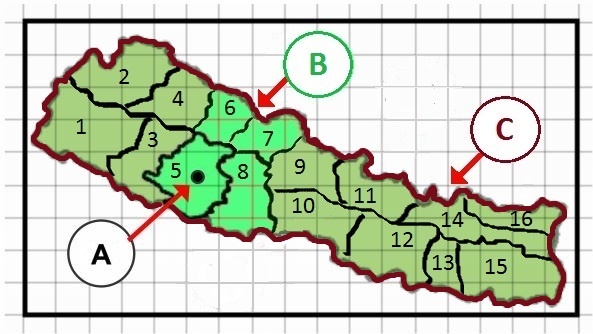
\includegraphics{nepal_ex}
\caption{Hypothetical example of spatial imprecision in aid allocation.}\label{fig:nepalex}
\end{figure}

\begin{figure}[!htbp]
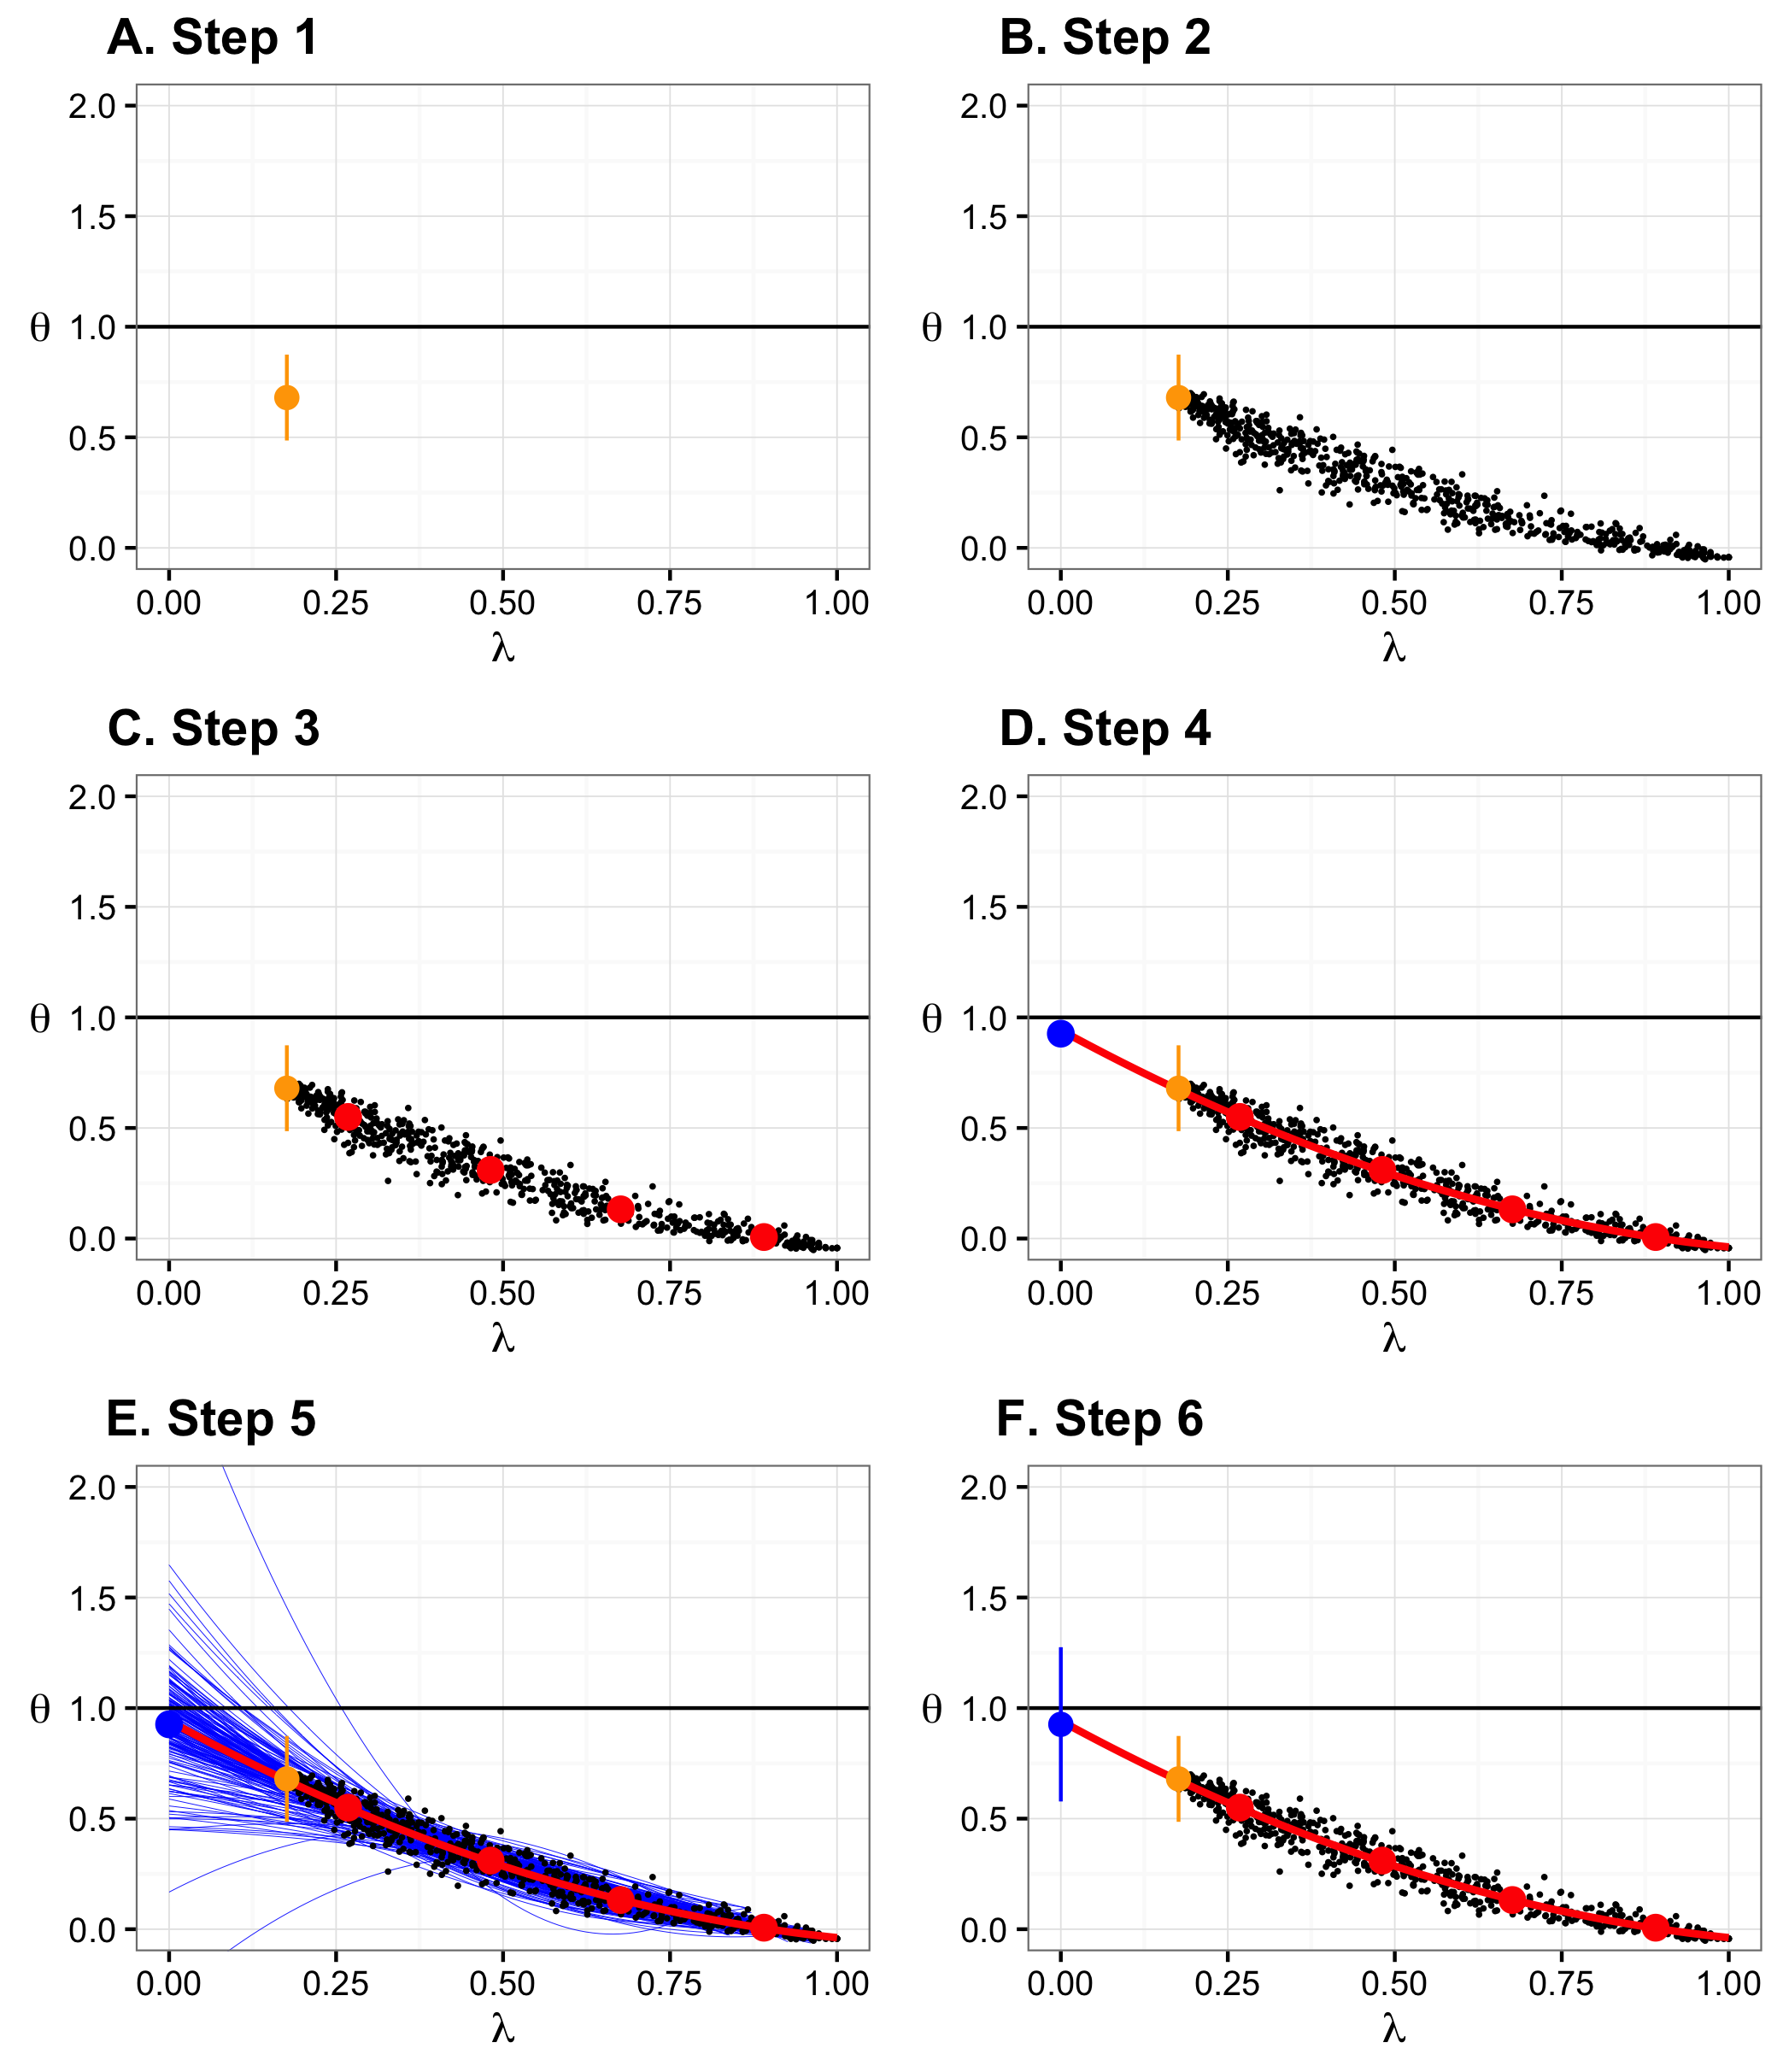
\includegraphics{steps}
\caption{Steps of the geoSIMEX procedure.}\label{fig:steps}
\end{figure}

%\begin{figure}[!htbp]
%\caption{Study area and units of observation.}\label{fig:studyarea}
%\end{figure}

\begin{figure}[!htbp]
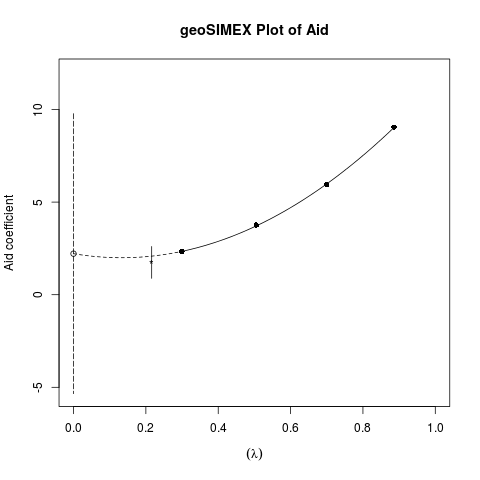
\includegraphics{geoSIMEX_plot.png}
\caption{geoSIMEX Plot of Aid.}\label{fig:geoSIMEX_plot}
\end{figure}

\newpage

%Acknowledgements
\section{Acknowledgements}
This work was performed in part using computational facilities at the College of William and Mary which were provided with the assistance of the National Science Foundation, Virginia Port Authority, Virginia Commonwealth Technology Research Fund, and the Office of Naval Research. 
The authors would also like to thank Ben Dykstra and Miranda Lv for their valuable insights.
\newpage

%Bibliography
\printbibliography

\end{document}
